\section{Training Details}

\subsection{Learning Rate}\label{app:lr}

Table~\ref{tab:learning_rate} lists learning rate configs for each model. For \VIT and \CONV, we have $\text{warmup}=500$. For \CROP, we don't have warmup steps.

\begin{table}[ht]
    \centering
    \begin{tabular}{c|cccc}
    \toprule
       \textbf{Model} & \textbf{Learning Rate}\tablefootnote{Intial learning rate, do not include warmup. So the actual Intial learning rate is $\frac{\text{Learning Rate}}{\text{Warmup Steps}}$.} & \textbf{Scheduler} & \textbf{Details} \\
    \midrule
        \VIT & $10^{-4}$ & ReduceLROnPlateau & $\begin{cases}\text{patience}=10\\\text{factor}=0.5\\\text{min\_lr}=5\times 10^{-6}\end{cases}$  \\
    \midrule
        \CONV & $10^{-4}$ & CosineAnnealingWarmRestarts & $\text{num\_cycles} = 0.5$\\
    \midrule
        \CROP & $10^{-5}$ & ReduceLROnPlateau & $\begin{cases}\text{patience}=5\\\text{factor}=0.5\\\text{min\_lr}=10^{-8}\end{cases}$  \\
    \bottomrule
    \end{tabular}
    \caption{Learning Rates Details for Each Models}
    \label{tab:learning_rate}
\end{table}

\subsection{LoRA Cofig}

In model selection period, we performed low-rank adaptation (LoRA) \cite{hu2021lora} for all experiments. We used the same LoRA config for all models to achieve the fairness.

We applied LoRA on all linear layers. Low rank matrices $A$ and $B$ are generated with the same method as in \cite{buyukakyuz2024olora}. The rank matrices are set to $8$, and the $\alpha$ parameter for LoRA scaling is set to $8$.

\subsection{Optimizer Config}\label{appendix:optimizer_config}

As section \ref{sec:finetuning_details} mentioned, we found no evidence that changing the optimizer affected the experimental results. So we use AdamW with hyperparameter $\beta_1=0.9, \beta_2=0.999, \epsilon=10^{-8}$ for all training processes.

\section{Submission Details}\label{app:submission_details}

We submitted our results to \href{https://www.kaggle.com/competitions/cassava-leaf-disease-classification/submissions}{Kaggle}.

Our final submission code can be found \href{https://github.com/pufanyi/SC4000/blob/main/submission/final_submission.ipynb}{here}.

Our final submission achieved $90.95\%$ (Rank $4 / 3901$, Top $0.10\%$) on Public Benchmark and $90.60\%$ (Rank $2 / 3901$, Top $0.05\%$) on Private Benchmark, shown in Figure \ref{fig:submission}, \ref{fig:public_lb} and \ref{fig:private_lb}.

\begin{figure}[H]
    \centering
    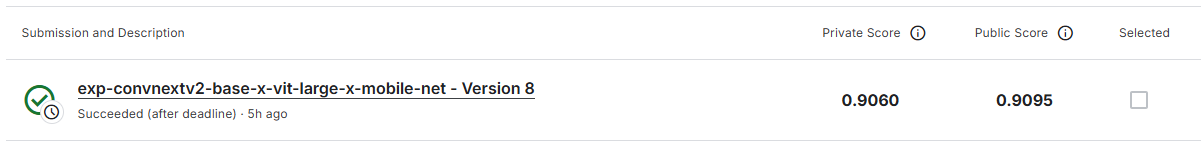
\includegraphics[width=1\linewidth]{graphs/appendix/results.png}
    \caption{Submission Results}
    \label{fig:submission}
\end{figure}

\begin{figure}[H]
    \centering
    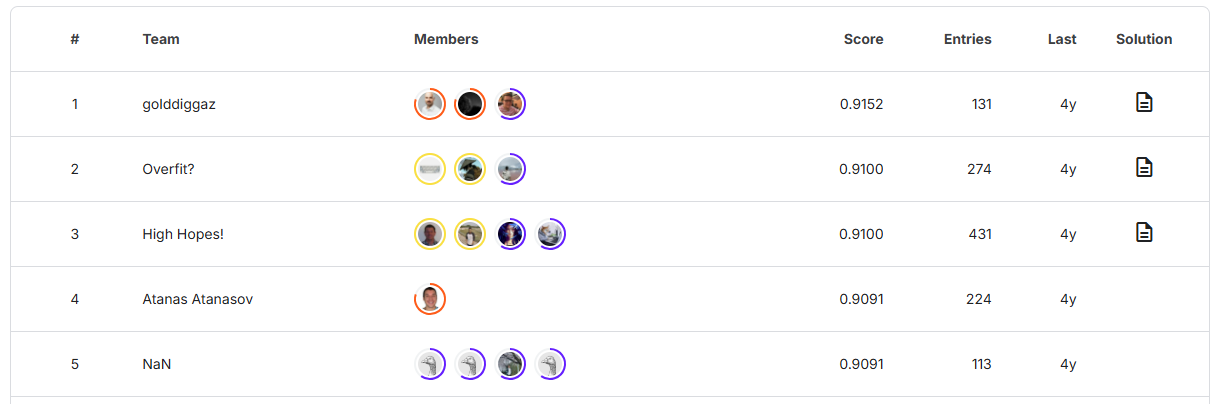
\includegraphics[width=1\linewidth]{graphs/appendix/publiclb.png}
    \caption{Public Leaderboard}
    \label{fig:public_lb}
\end{figure}

\begin{figure}[H]
    \centering
    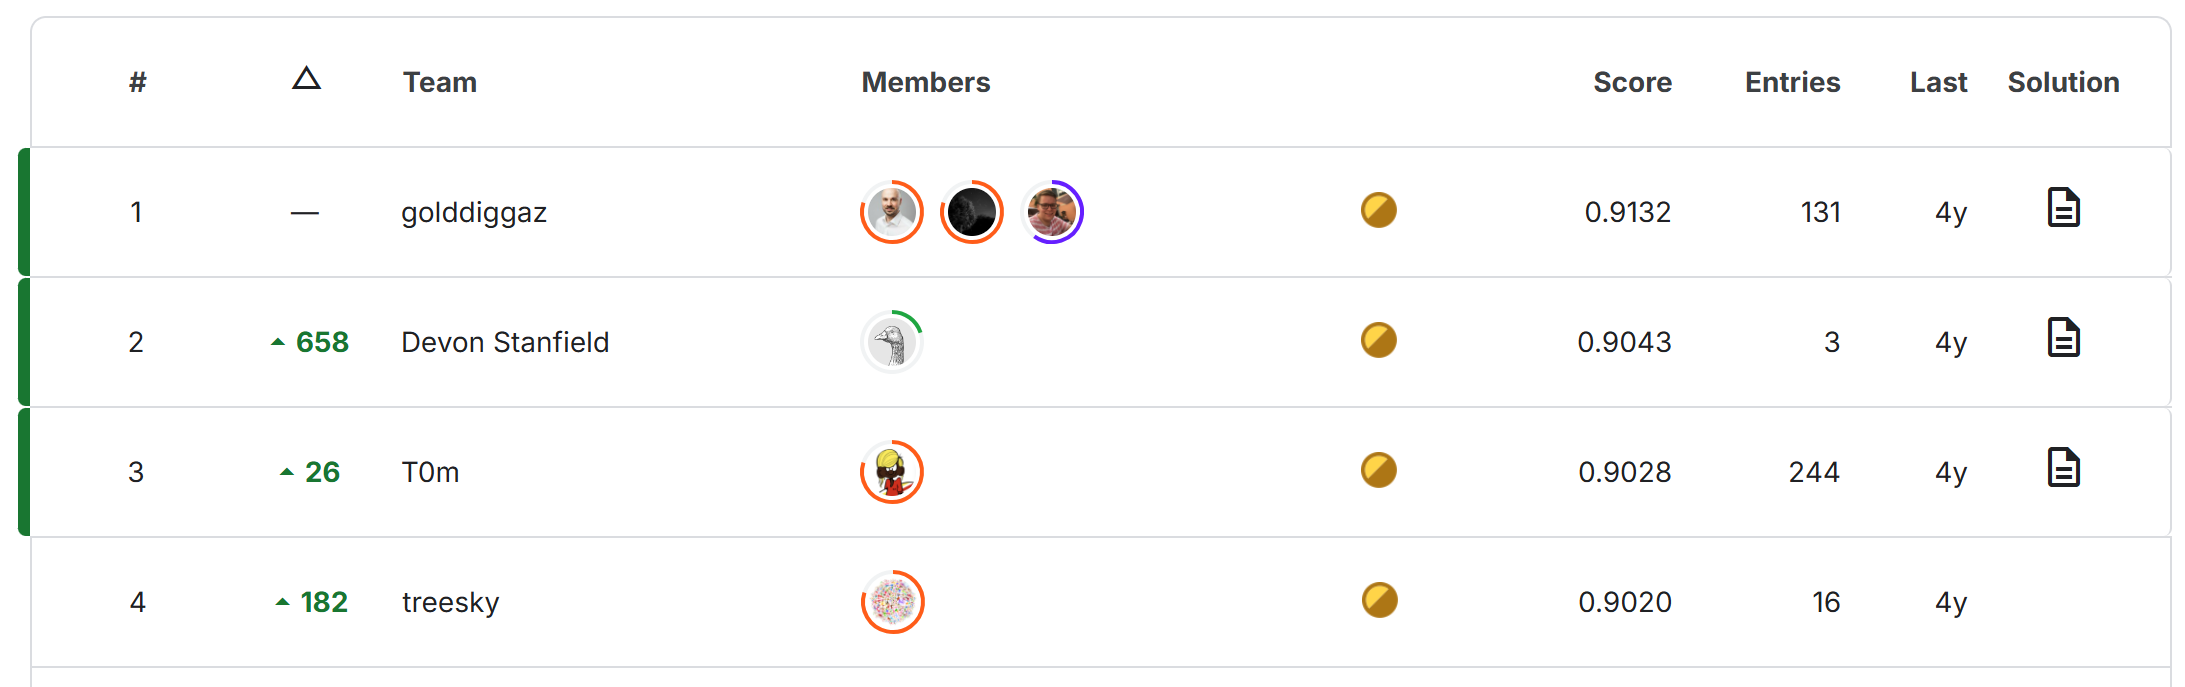
\includegraphics[width=1\linewidth]{graphs/appendix/privatelb.png}
    \caption{Private Leaderboard}
    \label{fig:private_lb}
\end{figure}
